\documentclass[hidelinks,12pt]{article}
\usepackage[left=0.25cm,top=1cm,right=0.25cm,bottom=1cm]{geometry}
%\usepackage[landscape]{geometry}
\textwidth = 20cm
\hoffset = -1cm
\usepackage[utf8]{inputenc}
\usepackage[spanish,es-tabla, es-lcroman]{babel}
\usepackage[autostyle,spanish=mexican]{csquotes}
\usepackage[tbtags]{amsmath}
\usepackage{nccmath}
\usepackage{amsthm}
\usepackage{amssymb}
\usepackage{mathrsfs}
\usepackage{graphicx}
\usepackage{subfig}
\usepackage{caption}
%\usepackage{subcaption}
\usepackage{standalone}
\usepackage[outdir=./Imagenes/]{epstopdf}
\usepackage{siunitx}
\usepackage{physics}
\usepackage{color}
\usepackage{float}
\usepackage{hyperref}
\usepackage{multicol}
\usepackage{multirow}
%\usepackage{milista}
\usepackage{anyfontsize}
\usepackage{anysize}
%\usepackage{enumerate}
\usepackage[shortlabels]{enumitem}
\usepackage{capt-of}
\usepackage{bm}
\usepackage{mdframed}
\usepackage{relsize}
\usepackage{placeins}
\usepackage{empheq}
\usepackage{cancel}
\usepackage{pdfpages}
\usepackage{wrapfig}
\usepackage[flushleft]{threeparttable}
\usepackage{makecell}
\usepackage{fancyhdr}
\usepackage{tikz}
\usepackage{bigints}
\usepackage{menukeys}
\usepackage{tcolorbox}
\tcbuselibrary{breakable}
\usepackage{scalerel}
\usepackage{pgfplots}
\usepackage{pdflscape}
\pgfplotsset{compat=1.16}
\spanishdecimal{.}
\renewcommand{\baselinestretch}{1.5} 
\renewcommand\labelenumii{\theenumi.{\arabic{enumii}})}

\newcommand{\python}{\texttt{python}}
\newcommand{\textoazul}[1]{\textcolor{blue}{#1}}
\newcommand{\azulfuerte}[1]{\textcolor{blue}{\textbf{#1}}}
\newcommand{\funcionazul}[1]{\textcolor{blue}{\textbf{\texttt{#1}}}}

\newcommand{\pderivada}[1]{\ensuremath{{#1}^{\prime}}}
\newcommand{\sderivada}[1]{\ensuremath{{#1}^{\prime \prime}}}
\newcommand{\tderivada}[1]{\ensuremath{{#1}^{\prime \prime \prime}}}
\newcommand{\nderivada}[2]{\ensuremath{{#1}^{(#2)}}}


\newtheorem{defi}{{\it Definición}}[section]
\newtheorem{teo}{{\it Teorema}}[section]
\newtheorem{ejemplo}{{\it Ejemplo}}[section]
\newtheorem{propiedad}{{\it Propiedad}}[section]
\newtheorem{lema}{{\it Lema}}[section]
\newtheorem{cor}{Corolario}
\newtheorem{ejer}{Ejercicio}[section]

\newlist{milista}{enumerate}{2}
\setlist[milista,1]{label=\arabic*)}
\setlist[milista,2]{label=\arabic{milistai}.\arabic*)}
\newlength{\depthofsumsign}
\setlength{\depthofsumsign}{\depthof{$\sum$}}
\newcommand{\nsum}[1][1.4]{% only for \displaystyle
    \mathop{%
        \raisebox
            {-#1\depthofsumsign+1\depthofsumsign}
            {\scalebox
                {#1}
                {$\displaystyle\sum$}%
            }
    }
}
\def\scaleint#1{\vcenter{\hbox{\scaleto[3ex]{\displaystyle\int}{#1}}}}
\def\scaleoint#1{\vcenter{\hbox{\scaleto[3ex]{\displaystyle\oint}{#1}}}}
\def\scaleiiint#1{\vcenter{\hbox{\scaleto[3ex]{\displaystyle\iiint}{#1}}}}
\def\bs{\mkern-12mu}

\newcommand{\Cancel}[2][black]{{\color{#1}\cancel{\color{black}#2}}}


\usepackage{minted}

\author{M. en C. Gustavo Contreras Mayén. \texttt{gux7avo@ciencias.unam.mx}}
\title{Evaluación del Examen Final \\ {\large Curso Física Computacional}}
\date{ }
\begin{document}

\maketitle
\fontsize{14}{14}\selectfont

\section{Problema 1.}
\begin{enumerate}
\item En tu función:
\begin{minted}{python}
def S1(N):
    suma1 = 0
    sumas1 = []
    for i in range(1,2*N):
        suma1 = suma1 + (-1)**i * i / (i+1)
        if i%2 == 0:
            sumas1.append(suma1)
    return suma1, sumas1
\end{minted}
Realizas la operación y luego revisar si el índice es par, cuando podrías dejar la operación dentro del condicional, no hay una \enquote{ganancia} computacional, si $N = \num{d4}$, se hacen ese mismo número de operaciones pero en el objeto \texttt{sumas1} solo hay la mitad de elementos.
\item ¿Para qué calcular el total de la suma? Es decir: \texttt{suma1}, ya que no se ocupa en alguna parte posterior de tu solución.
\item Te recomiendo separar las gráficas del error, ya que cada una muestra distintos comportamientos. Es claro que no se indicó de manera expresa, pero se sugiere interpretar cada una de manera aparte.
\item Tu comentario dentro del código sobre el comportamiento de cada gráfica es en parte correcto, pero ¿qué tiene que ver el error por redondeo entre las cantidades?
\item \textbf{Calificación: 0.9 puntos}
\end{enumerate}

\section{Problema 2.}

\begin{enumerate}
\item En tu función para el método de la falsa posición modificada, habría que comentar necesariamente lo que hace el método, es decir, bajo tu código no me queda claro por qué usas la variable \texttt{cambio}, que inicializas con un valor $0$, pero luego lo cambias a una cadena, me parece que es una bandera con la que identificas un extremo, pero al no haber un comentario al respecto, si sería necesario aclararlo.
\item ¿Por qué una tolerancia del orden de $\num{d-9}$? ¿Un valor mayor no garantiza la convergencia de tu método?
\item La solución en cada inciso con su gráfica está bien.
\item \textbf{Calificación: 0.9 puntos}
\end{enumerate}

\section{Problema 3.}

\begin{enumerate}
\item Mencionas que utilizaste el método del trapecio ya que por otros métodos, podría tardar bastante: ¿qué metodos utilizaste previamente? ¿en cuánto tiempo se redujo el cálculo?
\item \textbf{Calificación: 1 punto.}
\end{enumerate}

\section{Problema 4.}

\begin{enumerate}
\item Es mucho mejor definir un valor con notación científica $1e-7$ que utilizar $10**(-7)$.
\item Habiendo varios métodos de integración, ¿por qué elegiste Simpson $1/3$?
\item Bien por la gráfica con la solución.
\item Cuando presentas el valor de la energía, falta anotar las correspondientes unidades!!
\item \textbf{Calificación: 0.9 puntos.}
\end{enumerate}

\section{Problema 5.}

\begin{enumerate}
\item Cuando mencionas que elegiste Rk4 por que es más eficiente, preciso y que no ocupa tantos recursos computacionales como otros métodos, que no aclaras cuáles, puedes referirte en términos del error asociado, pero hay un método el adaptativo que es un método que mejora el resultado, pero ¿deja de ser eficiente?
\item Bien por las gráficas.
\item \textbf{Calificación: 1 punto.}
\end{enumerate}

\section{Problema 6.}

\begin{enumerate}
\item Bien por el planteamiento que presentas.
\item Los límites para las gráficas ¿son necesarios? El problema pide que calcules un valor para $30$ días, pero no quiere decir que la gráfica quede limitada también.
\item En los resultados en la terminal si bien presentas lo que se supone son $x (30)$, $y (40)$ y $z (30)$ no se reconoce cuál es cuál, es decir, necesitas identificar cada valor.
\item En el inciso 6.2 a partir del cambio de variable que se sugiere, también se pregunta por el significado del valor límite cuando $t \to \infty$, pero respondes la pregunta.
\item \textbf{Calificación: 0.9}
\end{enumerate}

\section{Problema 7.}

\begin{enumerate}
\item Bien por el planteamiento del sistema de ecuaciones algebraico para los dos incisos.
\item Bien por el código que resuelve el sistema tridiagonal.
\item Para el inciso 7.2, ¿no hubo solución exacta para comparar el resultado?
\item \textbf{Calificación: 1 punto.}
\end{enumerate}

\section{Problema 8.}

\begin{enumerate}
\item En tu discusión inicial para aproximar la función a integrar, planteas una estrategia que se revisó en otro ejercicio, está bien, pero está mejor que hicieras una revisión previa de esa función, si hubieras graficado la misma, te hubieras dado cuenta del valor con el cual puedes dar por sentado el comportamiento de la función, en este caso, para los dos incisos:
\begin{figure}[H]
    \centering
    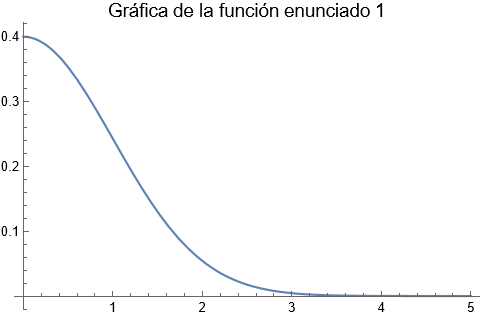
\includegraphics[scale=0.8]{plot_P1_Inciso_01.png}
    \caption{Puedes ver que no había que discutir mucho por el intervalo superior de integración.}
\end{figure}
\begin{figure}[H]
    \centering
    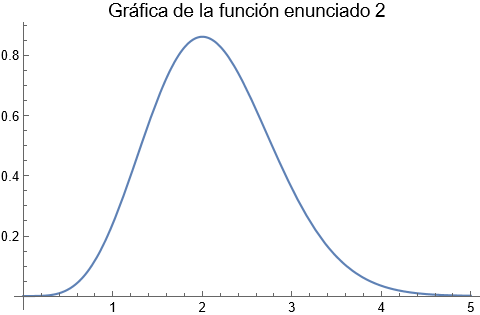
\includegraphics[scale=0.8]{plot_P1_Inciso_02.png}
    \caption{Para el segundo inciso ocurre lo mismo, el valor del intervalo superior de integración se intuye de manera directa.}
\end{figure}
\item Desarrollas una función para el manejo de los valores aleatorios, que bien te resuelve lo que se pide en el ejercicio.
\item \textbf{No} reportas en la terminal el valor de la integral obtenida.
\item En las gráficas que se generan no queda claro qué es lo que presentas: en una mencionas que se muestra el error relativo contra el número de iteraciones, pero la segunda gráfica dice en el título que es el valor de la integral y no es lo que se muestra.
\item El valor exacto de cada integral lo conoces por el enunciado, no entiendo por que en tu función de error ocupas un radical con $\pi$.
\item Al utilizar este método y con un valor de $n$ distinto, se esperaba también la gráfica de puntos por debajo de la curva y por arriba de la misma, como se hizo con el método del dardo. Pero no están estas gráficas.
\item \textbf{Calificación: 0.6 puntos.}
\end{enumerate}

\section{Problema 9}.

\begin{enumerate}
\item Conviene bastante que comentes el qué es lo que haces y por qué propones un código como el que presentas.
\item La idea es buena, ya que consideras la geometría del ejercicio, pero no explicas que vas a calcular una cuarta parte del volumen del hemisferio, para que con el valor que te resulte, luego lo multiplicas por $4$ y con ello, la aproximación del volumen es lo que presentas.
\item Este tipo de revisión previa te ayuda mucho para explicar en una evaluación que es lo que hiciste y para qué.
\item El valor exacto del volumen, bien podrías haber hecho la cuenta de Cálculo IV para obtener el volumen del hemisferio, que si es el que indicas, pero mostrar ese valor como algo ya hecho, le resta a tu solución.
\item \textbf{Calificación: 0.9 puntos.}
\end{enumerate}



\end{document}